\documentclass[a4paper,12pt]{article}

%%% Работа с русским языком
\usepackage{cmap}					% поиск в PDF
\usepackage{mathtext} 				% русские буквы в формулах
\usepackage[T2A]{fontenc}			% кодировка
\usepackage[utf8]{inputenc}			% кодировка исходного текста
\usepackage[english,russian]{babel}	% локализация и переносы
\usepackage{xcolor}
\usepackage{hyperref}
 % Цвета для гиперссылок
\definecolor{linkcolor}{HTML}{799B03} % цвет ссылок
\definecolor{urlcolor}{HTML}{799B03} % цвет гиперссылок

\hypersetup{pdfstartview=FitH,  linkcolor=linkcolor,urlcolor=urlcolor, colorlinks=true}

%%% Дополнительная работа с математикой
\usepackage{amsfonts,amssymb,amsthm,mathtools} % AMS
\usepackage{amsmath}
\usepackage{icomma} % "Умная" запятая: $0,2$ --- число, $0, 2$ --- перечисление

%% Номера формул
%\mathtoolsset{showonlyrefs=true} % Показывать номера только у тех формул, на которые есть \eqref{} в тексте.

%% Шрифты
\usepackage{euscript}	 % Шрифт Евклид
\usepackage{mathrsfs} % Красивый матшрифт

%% Свои команды
\DeclareMathOperator{\sgn}{\mathop{sgn}}

%% Перенос знаков в формулах (по Львовскому)
\newcommand*{\hm}[1]{#1\nobreak\discretionary{}
{\hbox{$\mathsurround=0pt #1$}}{}}
% графика
\usepackage{graphicx}
\graphicspath{{pictures/}}
\DeclareGraphicsExtensions{.pdf,.png,.jpg}
\author{Бурмашев Григорий, БПМИ-208}
\title{ТВиМС, дз -- какое-то}
\date{\today}
\begin{document}
\maketitle
\clearpage
\section*{Номер 1}
У $X$ распределение $\text{Exp}(q)$. Для начала посмотрим на хар.функцию для самой $X$:
\[
\varphi_X(a) = \frac{q}{q - ia}
\]
Теперь смотрим на хар.функцию для $X \cdot q$:
\[
\varphi_{X \cdot q}(t) = \varphi_X (tg) \cdot e^{it0} = \varphi_X(tg)=  \frac{q}{q - itg} = \frac{1}{1 - it} = \text{Exp}(1)
\]
\section*{Номер 5 [листок 2]}
\subsection*{b)}
\[
(\text{Im} \varphi(t))^2 \leq \frac{1}{2} \left(1 - \text{Re} \varphi(2t)\right) \; ?
\]
Проверяем:
\[
\left(
 \text{Im} \left(
\mathbb{E} \cos (Xt) + i \mathbb{E} \sin (Xt)
\right)
 \right)^2
\leq  
\frac{1}{2}
 \left(
1 - \text{Re}
\left(
\mathbb{E} \cos (2Xt) + i \mathbb{E} \sin (2Xt)
\right)
\right)
\]
\[
\left( \mathbb{E} \sin (Xt) \right)^2 \leq \frac{1}{2} \left(
1 - \mathbb{E} \cos (2 X t)
\right)
\]
\[
\left( \mathbb{E} \sin (Xt) \right)^2 \leq \frac{1}{2} \left(
1 - \mathbb{E} \cos (1 - 2 \sin^2 (Xt)) 
\right)
\leq
\frac{1}{2} E \sin^2 (Xt)
\]
\[
\left( \mathbb{E} \sin (Xt) \right)^2   \leq \frac{1}{2} E \sin^2 (Xt)
\]
Ну а это верно как свойство математического ожидания
\begin{center}
\textbf{Ч.Т.Д} 
\end{center}
\subsection*{c)}
\[
\left(
\text{Re} \varphi(t)
\right)^2 
\leq
\frac{1}{2}
\left(
1 + \text{Re}\varphi(2t)
\right) \; ?
\]
Проверяем:
\[
\mathbb{E}^2 \cos (Xt) \leq \frac{1}{2} \left(
1 + \mathbb{E} \cos (2Xt)
\right) \leq \frac{1}{2} + \frac{1}{2} \mathbb{E} \left(2 \cos^2 (Xt) - 1\right) \leq E \left(\cos^2 (Xt)\right)
\]
Ну а это верно как свойство математического ожидания
\begin{center}
\textbf{Ч.Т.Д} 
\end{center}
\clearpage
\section*{Номер 8 [листок 3]}
\begin{center}

\includegraphics[scale=0.4]{3.png}
\end{center}
Представим наше подбрасывание (взял под копирку с семинара 2010):
\[
I_6 -- \text{ индикатор того, что выпало 6 }
\]
\[
X = \sum_{i = 1}^{12000} I_6
\]
\[
\mathbb{E}I_6 = P(\text{выпало 6}) = \frac{1}{6}
\]
\[ 
\mathbb{D}I_6 = \mathbb{E}I_6^2 - (\mathbb{E}I_6)^2 = \frac{1}{6} - \frac{1}{6^2} = \frac{5}{36}
\]
Отсюда
\[
\sigma(I_6) = \sqrt{\frac{5}{36}}
\]
Ну а по условию задачи мы хотим найти:
\[
P
\left(
1800 \leq  \sum_{i = 1}^{12000} I_6 \leq 2100
\right)
\]
Применяем ЦПТ и получаем:
\[
P
\left(
1800 \leq  \sum_{i = 1}^{12000} I_6 \leq 2100
\right) =
P 
\left(
\frac{\sum\limits_{k = 1}^{1800}I_6 - \frac{12000}{6}}{\sqrt{12000 \cdot \frac{5}{36}}} 
\leq
\frac{\sum\limits_{k = 1}^{12000}I_6 - \frac{12000}{6}}{\sqrt{12000 \cdot \frac{5}{36}}} 
\leq
\frac{\sum\limits_{k = 1}^{2100}I_6 - \frac{12000}{6}}{\sqrt{12000 \cdot \frac{5}{36}}} 
\right) \sim
\]
\[
\sim
 \text{Ф}
\left(
\frac{2100 - \frac{12000}{6}}{\sqrt{12000 \cdot \frac{5}{36}}} 
\right)
-
 \text{Ф}
\left(
\frac{1800 - \frac{12000}{6}}{\sqrt{12000 \cdot \frac{5}{36}}} 
\right) =
\]
\[
=
 \text{Ф}
\left(
\frac{100}{\sqrt{\frac{5000}{3}}}
\right)
+
 \text{Ф}
\left(
\frac{200}{\sqrt{\frac{5000}{3}}}
\right)
=
\text{Ф}(\sqrt{6}) + \text{Ф}(2 \sqrt{6})
\]
\begin{center}
\textbf{Ответ: } 
\[
\text{Ф}(\sqrt{6}) + \text{Ф}(2 \sqrt{6})
\]
\end{center}
\clearpage
\section*{Номер 9 [листок 3]}
\begin{center}

\includegraphics[scale=0.4]{4.png}
\end{center}
Ну собственно таска аналог 5й с сема. Будем пользоваться теорией с сема:
\begin{center}
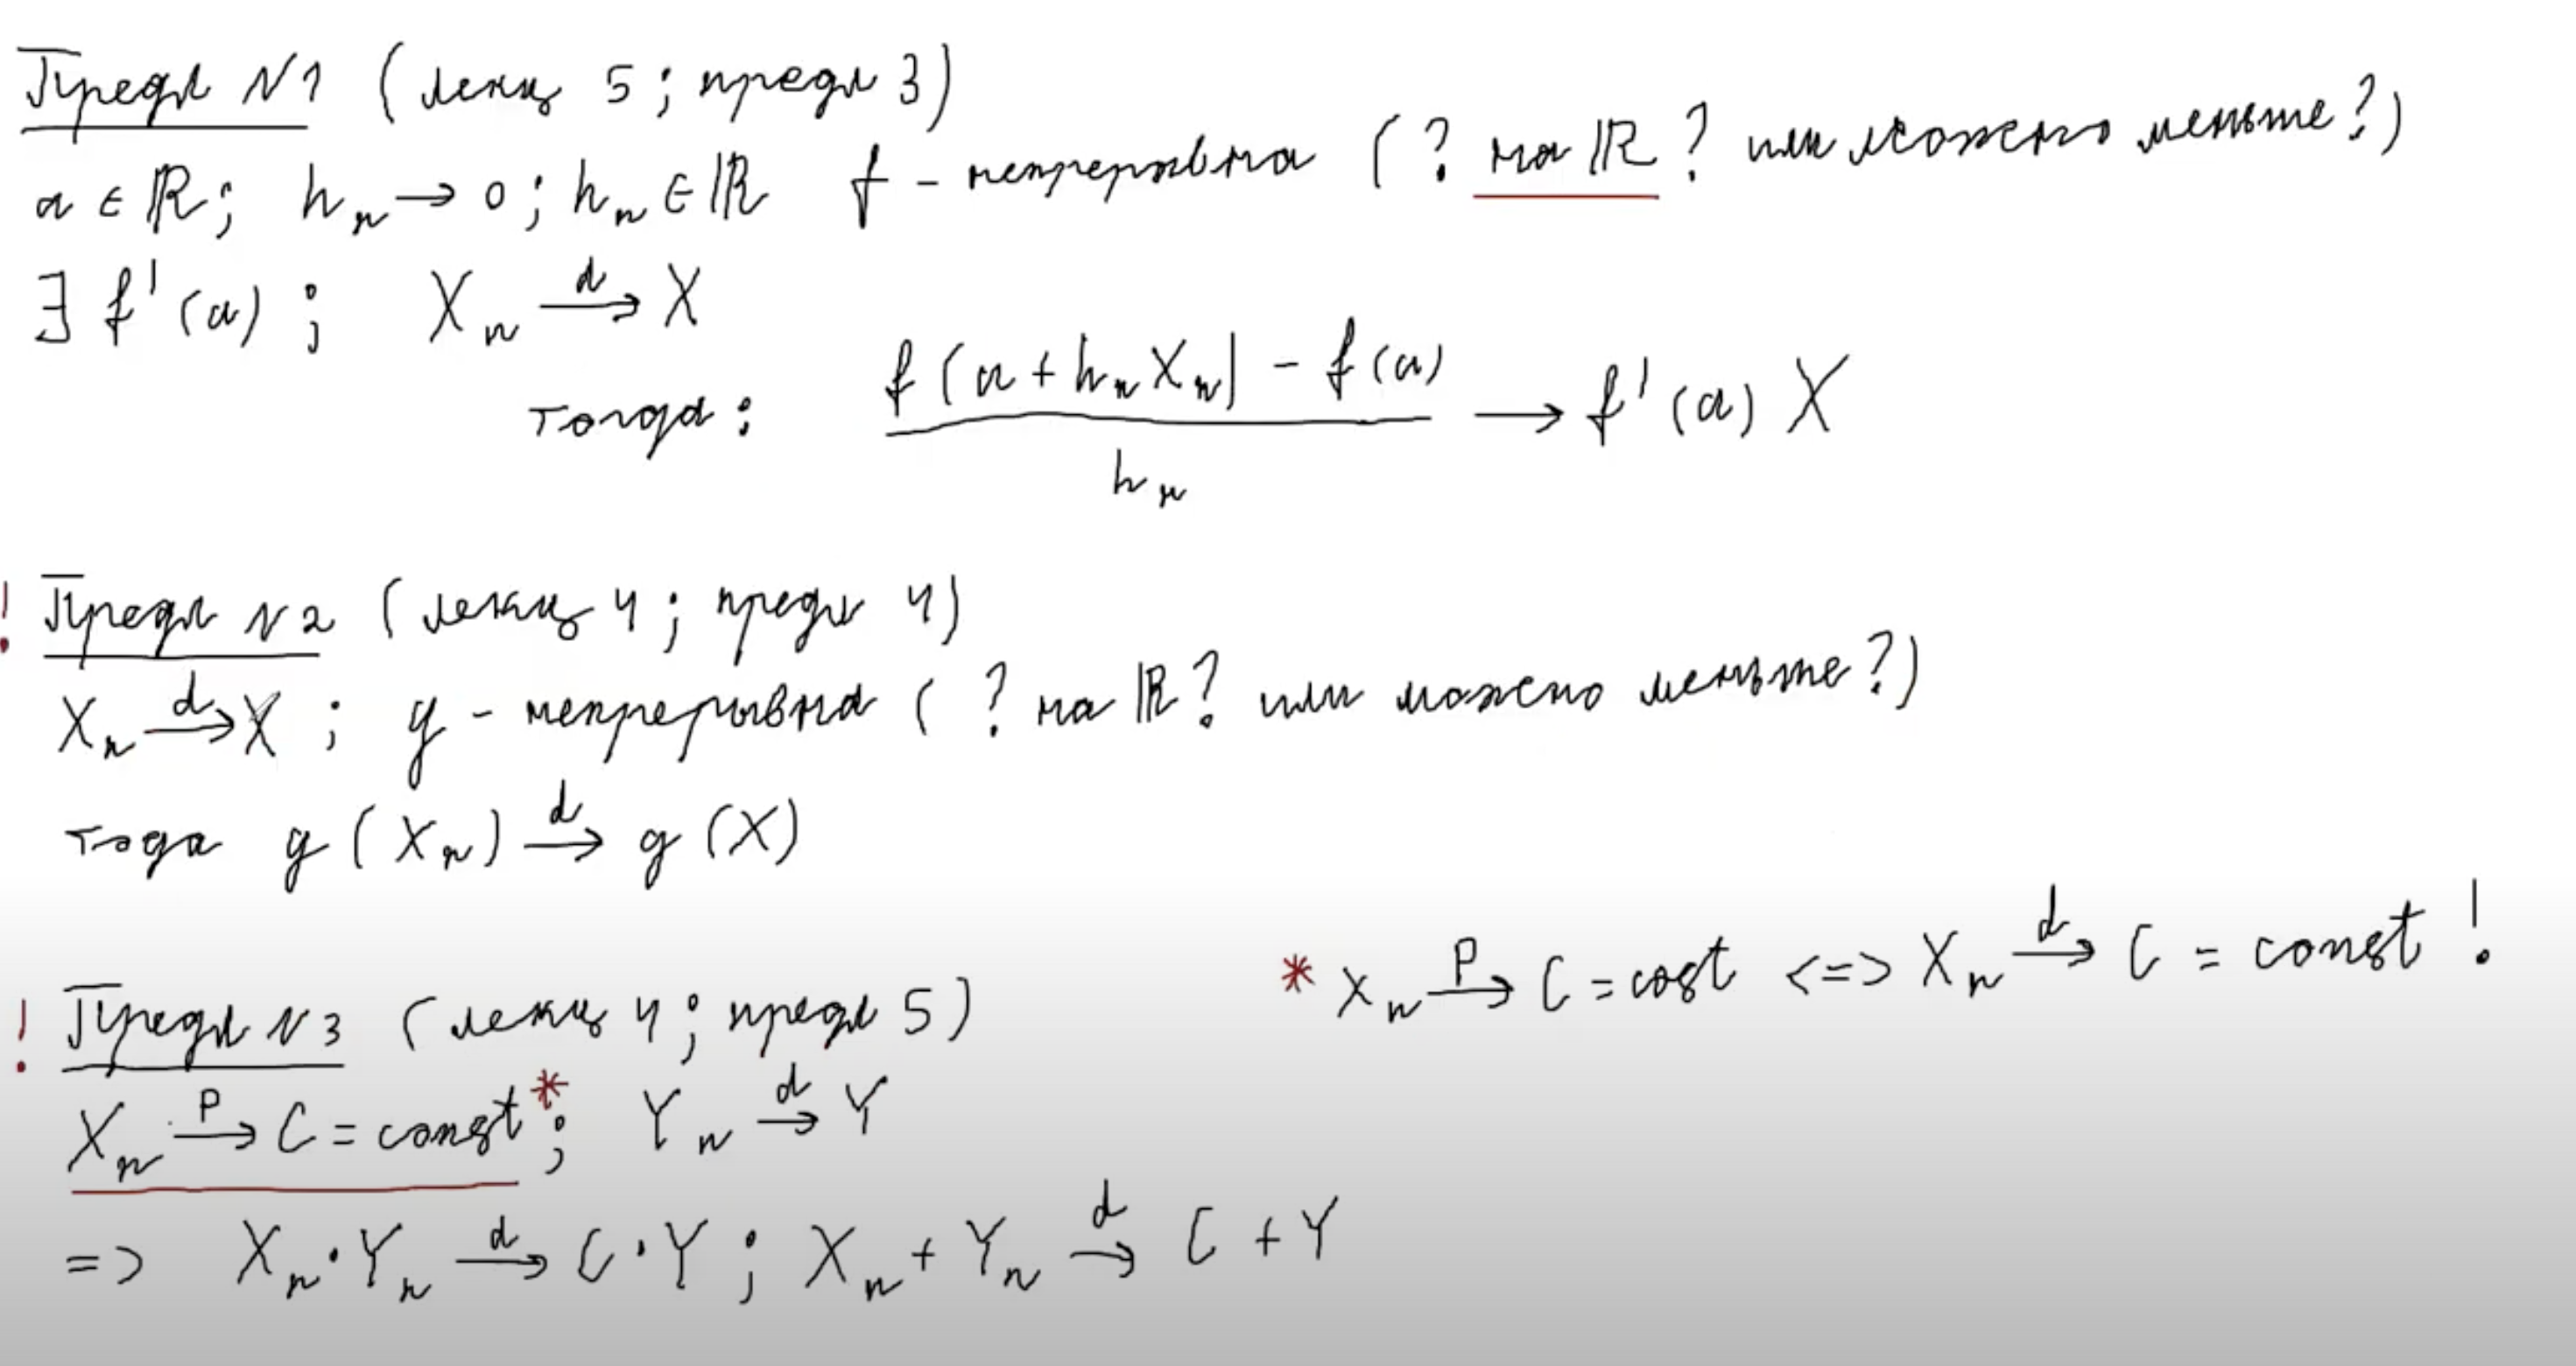
\includegraphics[scale=0.2]{5.png}
\end{center}
Приведем все к общему знаменателю:
\[
\sqrt{n} \left(
\frac{5}{4} \frac{V_n}{U_n} - a = 
\right)
=
\sqrt{n} 
\left(
\frac{5}{4}V_n - U_n \cdot a 
\right)
\cdot
\frac{n}{\sum\limits_{j=1}^{n} X_j^3}
\]
Заметим:
\[
\frac{Y_1 + \ldots + Y_n}{n}
\overset{P}{\longrightarrow} \mathbb{E}Y_k = \text{const}
\]
Если $Y_1, \ldots Y_n$ независимы, одинаково распределенны и $\mathbb{E}Y_k$ -- есть (ЗБЧ). Следовательно (из предл. 2 и предл. 3):
\[
\frac{n}{\sum\limits_{j = 1}^n X_j^3}\overset{P}{\longrightarrow} \frac{1}{\mathbb{E} X_i^3}
\]
А отсюда:
\[
\sqrt{n} 
\left(
\frac{5}{4}V_n - U_n \cdot a 
\right)
\cdot
\frac{n}{\sum\limits_{j=1}^{n} X_j^3} 
\overset{d}{\longrightarrow} \frac{Z}{\mathbb{E} X_i^3}
\]
Пусть:
\[
W_i = \frac{5}{4} X_i^4 - a X_i^3
\]
Ну и:
\[
\sum_{j = 1}^{n} W_j = \sum_{j = 1}^n \left(\frac{5}{4} X_j^4 - a X_j^3 \right)
\]
Тогда:
\[
\sqrt{n} 
\left(
\frac{5}{4}V_n - U_n \cdot a 
\right)
=
\frac{W_1 + \ldots + W_n}{\sqrt{n}}
=
\frac{W_1 + \ldots + W_n - n \mathbb{E} W_i}{\sqrt{n}} + \sqrt{n} \mathbb{E} W_i
\]
Заметим, что $\sqrt{n} \mathbb{E} W_i$ либо стремится к нулю, если $\mathbb{E} W_i = 0$, либо к бесконечности, если $\mathbb{E} W_i \neq 0$. А левая штука похожа на ЦПТ. Теперь считаем:
\[
\mathbb{E} W_i = \frac{5}{4} \mathbb{E}X_i^4 - a \mathbb{E}X_i^3
\]
\[
\mathbb{E}X_i^3 = \int\limits_{-\infty}^{+\infty} x^3 \cdot \frac{1}{a} \cdot I_{x \in [0, a]} = \frac{1}{a} \int\limits_0^a x^3 = \frac{a^3}{4}
\]

\[
\mathbb{E}W_i= \int\limits_{-\infty}^{+\infty} \left(
\frac{5}{4}X_i^4 - a \cdot X_i^4 
\right)
\cdot I_{x \in [0, a]} dx=
\frac{5}{4} \cdot \frac{x^5}{5} \Bigg|_0^a - a \cdot \frac{x^4}{4} \Bigg|_0^a = 0
\]
Смотрим:
\[
\frac{\sum_{i = 1}^n \left(W_i \right)- n \cdot \mathbb{E} W_i }{\sqrt{n}} + \sqrt{n} \mathbb{E} W_i = \sqrt{\mathbb{D}W_i} \cdot \frac{\sum_{i =1^n \left(W_i\right) - n \mathbb{E}W_i }}{\sqrt{n}} \overset{d}{\longrightarrow} \sqrt{\mathbb{D}W_i} \cdot \overline{Z} 
\]
Ну а:
\[
\overline{Z}  \sim N(0, 1)
\]
Тогда найдем:
\[
\mathbb{D}W_i  = \int\limits_0^a \left(
\frac{5}{4} x^4 - ax^3 
\right)^2dx = 
\]
\[
=
\frac{25}{16a} \int_0^a x^8dx - \frac{5}{2} \int_0^a x^7 dx + a \int_0^a x^6 dx = \frac{a^8}{252}
\]
Тогда:
\[
Z \cdot \frac{4}{a^3} \rightarrow 
N
\left(
0, \sqrt{\frac{a^8}{256}} \cdot \frac{4}{a^3} 
\right)
=
N
\left(
0, a \cdot \frac{2\sqrt{7}}{21}
\right)
\]
\begin{center}
\textbf{Ответ: } 
\[
\sqrt{n}
 \left(
\frac{5}{4}
\frac{V_n}{U_n} - 1
\right)
\overset{d}{\longrightarrow}
N
\left(
0, a \cdot \frac{2\sqrt{7}}{21}
\right)
\]
\end{center}
\end{document}
